\chapter{系统架构}

本文提出一个基于可编程网卡的高性能数据中心系统架构。
可编程网卡是服务器与外界通信的 ``网关'',也是服务器内硬件设备、虚拟机间通信的 ``枢纽''。
我们把虚拟化、网络和存储功能、操作系统中需要高性能的数据平面卸载到可编程网卡,以降低 ``数据中心税'',让 CPU 集中精力于客户的应用程序。


\begin{figure}[htbp]
	\centering
	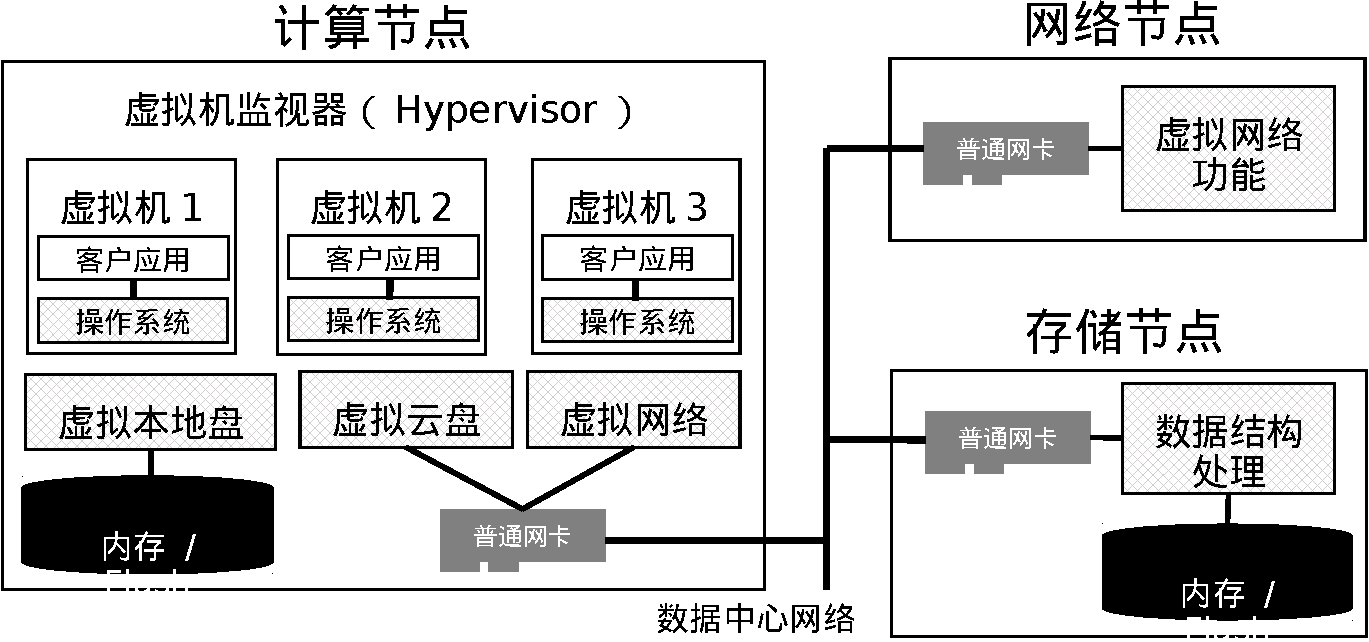
\includegraphics[width=0.8\textwidth]{figures/virt_arch.pdf}
	\caption{回顾:虚拟化的数据中心架构。}
	\label{arch:fig:virt-architecture}
\end{figure}

第 \ref{chapter:intro} 章已经讨论过,如图 \ref{arch:fig:virt-architecture} 所示,虚拟化的数据中心主要可以分为计算、网络、存储节点。
在网络和存储节点,我们采用控制面与数据面分离的设计思想。数据面是操作相对频繁、逻辑相对简单的处理,而控制面是操作相对不频繁、逻辑相对复杂的处理。我们在可编程网卡中实现数据面,在主机 CPU 上实现控制面,实现了数据面完全不经过主机 CPU。这包括第 \ref{chapter:clicknp} 章的虚拟网络功能和第 \ref{chapter:kvdirect} 章的数据结构处理。加速虚拟网络功能和远程数据结构访问也是本文最重要的创新。

在计算节点,亦即客户虚拟机所在的服务器主机上,我们用可编程网卡实现虚拟机监控器(hypervior)的虚拟化功能和操作系统原语。
虚拟化分为 ``一虚多'' 和 ``多虚一'' 两个方面。
``一虚多'',即可编程网卡把计算节点内的硬件资源虚拟化成多个逻辑资源,实现其他计算节点和本地多台虚拟机的多路复用。例如,第 \ref{chapter:clicknp} 章的 ClickNP 将硬件网卡和网络链路虚拟化为每个虚拟机一张虚拟网卡;第 \ref{chapter:clicknp} 章的 KV-Direct 实现了多个客户端并发访问共享键值存储,并能保证一致性。
``多虚一'',即可编程网卡把数据中心内物理上分散的资源虚拟化成一个逻辑资源,实现逻辑资源到物理资源的映射和路由。例如,第 \ref{chapter:clicknp} 章的 ClickNP 将数据中心内网络功能虚拟化成逻辑上统一的网络功能;第 \ref{chapter:clicknp} 章的 KV-Direct 客户端将分布式键值存储虚拟化成逻辑上统一的键值映射;还可以实现存储和内存的解聚(disaggregation)。
为了加速操作系统原语并控制硬件的复杂度,我们把操作系统原语划分为可编程网卡上的可靠通信协议和主机 CPU 上运行的用户态库、用户态管理程序,如第 \ref{chapter:socksdirect} 章 SocksDirect 实现的套接字通信原语。

图 \ref{arch:fig:accel-arch} 显示了基于可编程网卡的系统总体架构。下面我们将按照网络、存储和高层抽象的顺序,简要介绍本文后续各章的总体设计。


\begin{figure}[htbp]
	\centering
	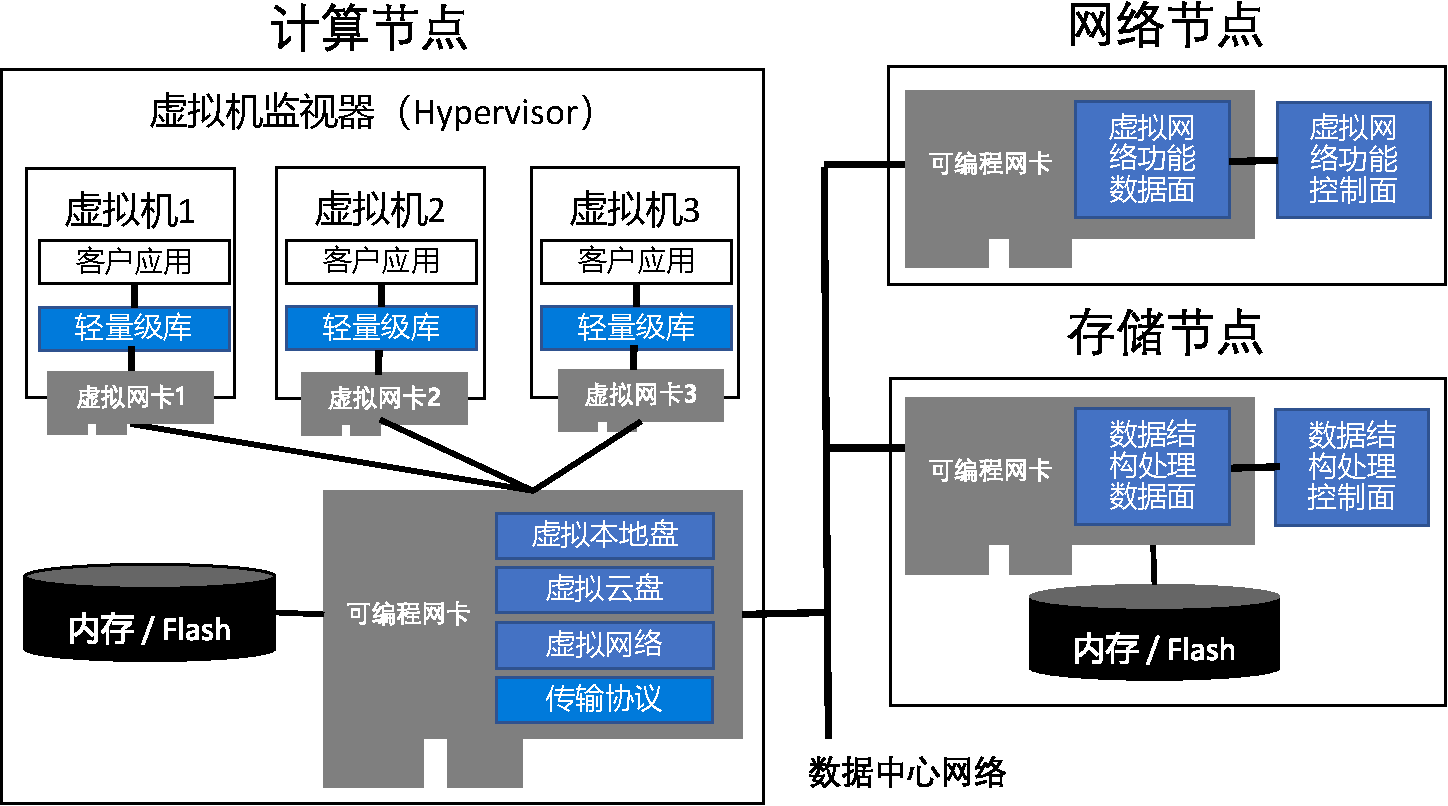
\includegraphics[width=0.8\textwidth]{figures/accel_arch.pdf}
	\caption{基于可编程网卡的数据中心系统总体架构。}
	\label{arch:fig:accel-arch}
\end{figure}



\section{网络加速}

\subsection{网络虚拟化加速}

第 \ref{chapter:clicknp} 章的 ClickNP 将硬件网卡和网络链路虚拟化为多个租户的虚拟网络;第 \ref{chapter:socksdirect} 章的 SocksDirect 实现了容器网络。

\begin{figure}[htbp]
	\centering
	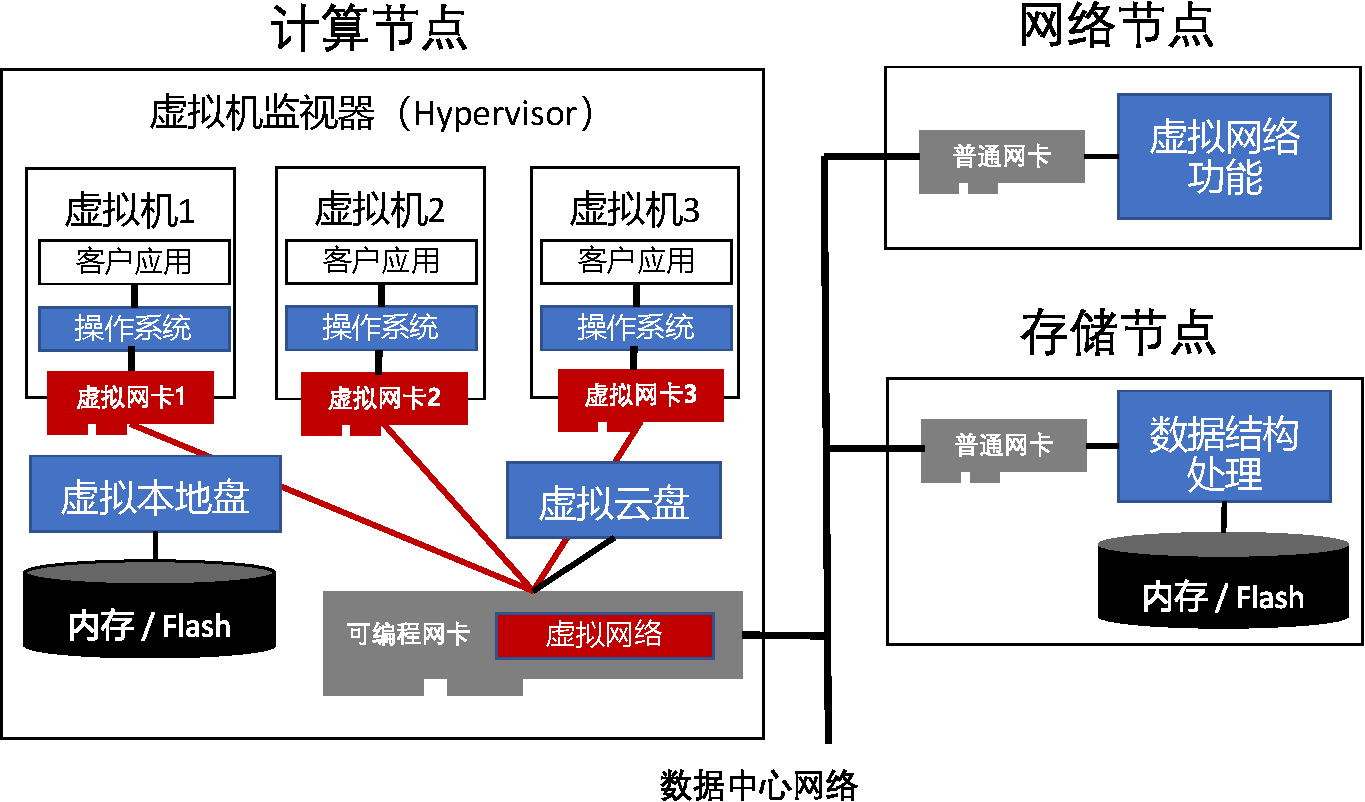
\includegraphics[width=0.8\textwidth]{figures/virtual_network.pdf}
	\caption{用可编程网卡加速虚拟网络后的架构。}
	\label{arch:fig:virtual-network}
\end{figure}

\subsection{网络功能加速}

我们在可编程网卡中实现数据面,在主机 CPU 上实现控制面,实现了数据面完全不经过主机 CPU。

直接处理网络数据包并直接返回,数据面无需经过 CPU(ClickNP NF offload)。


\begin{figure}[htbp]
	\centering
	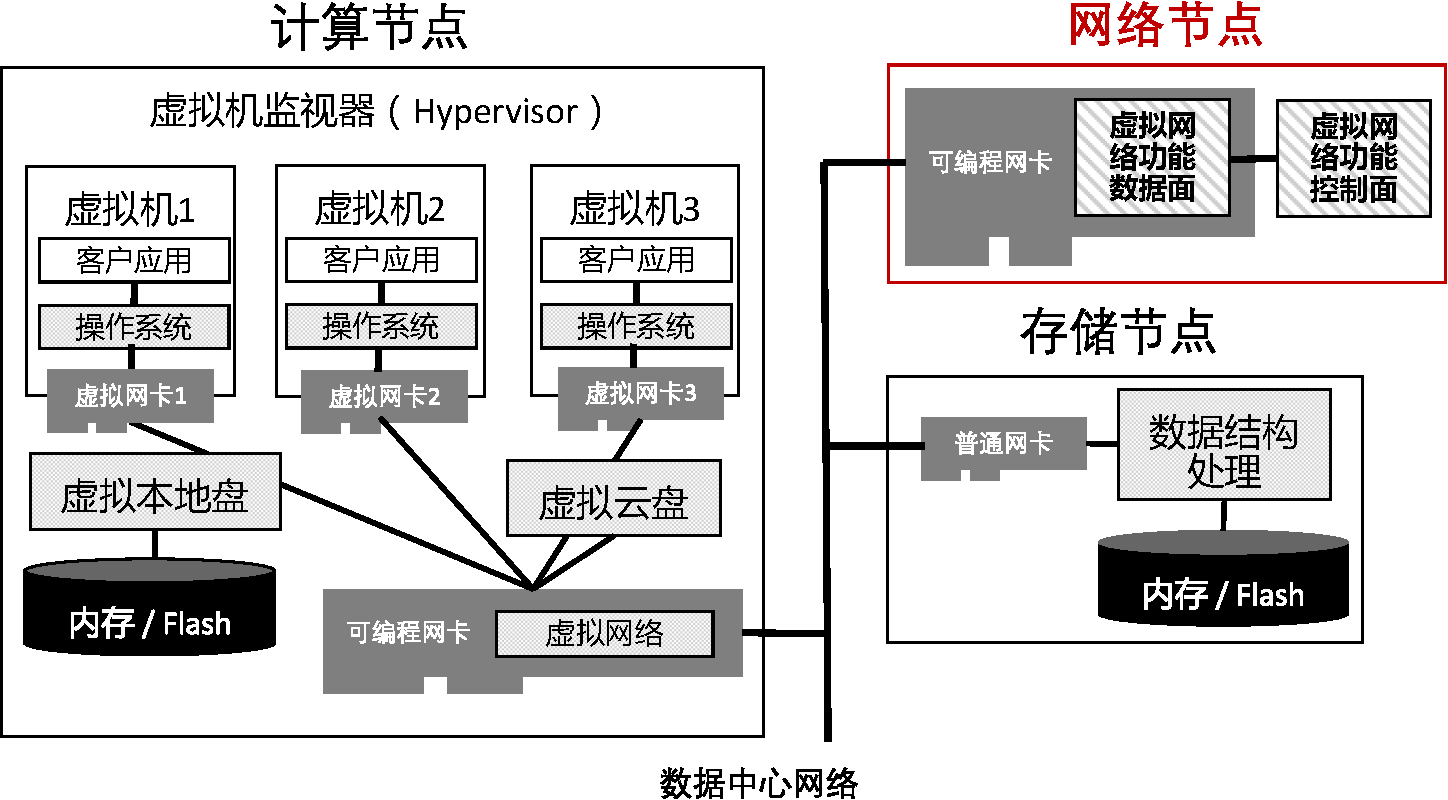
\includegraphics[width=0.8\textwidth]{figures/NFV_accel.pdf}
	\caption{用可编程网卡加速网络功能后的架构。}
	\label{arch:fig:network-function}
\end{figure}

\section{存储加速}

\subsection{存储虚拟化加速}

第 \ref{chapter:clicknp} 章的 KV-Direct 客户端将分布式键值存储虚拟化成一个大的哈希表;

不管是本地访问还是远程访问,都统一经过可编程网卡。

\begin{figure}[htbp]
	\centering
	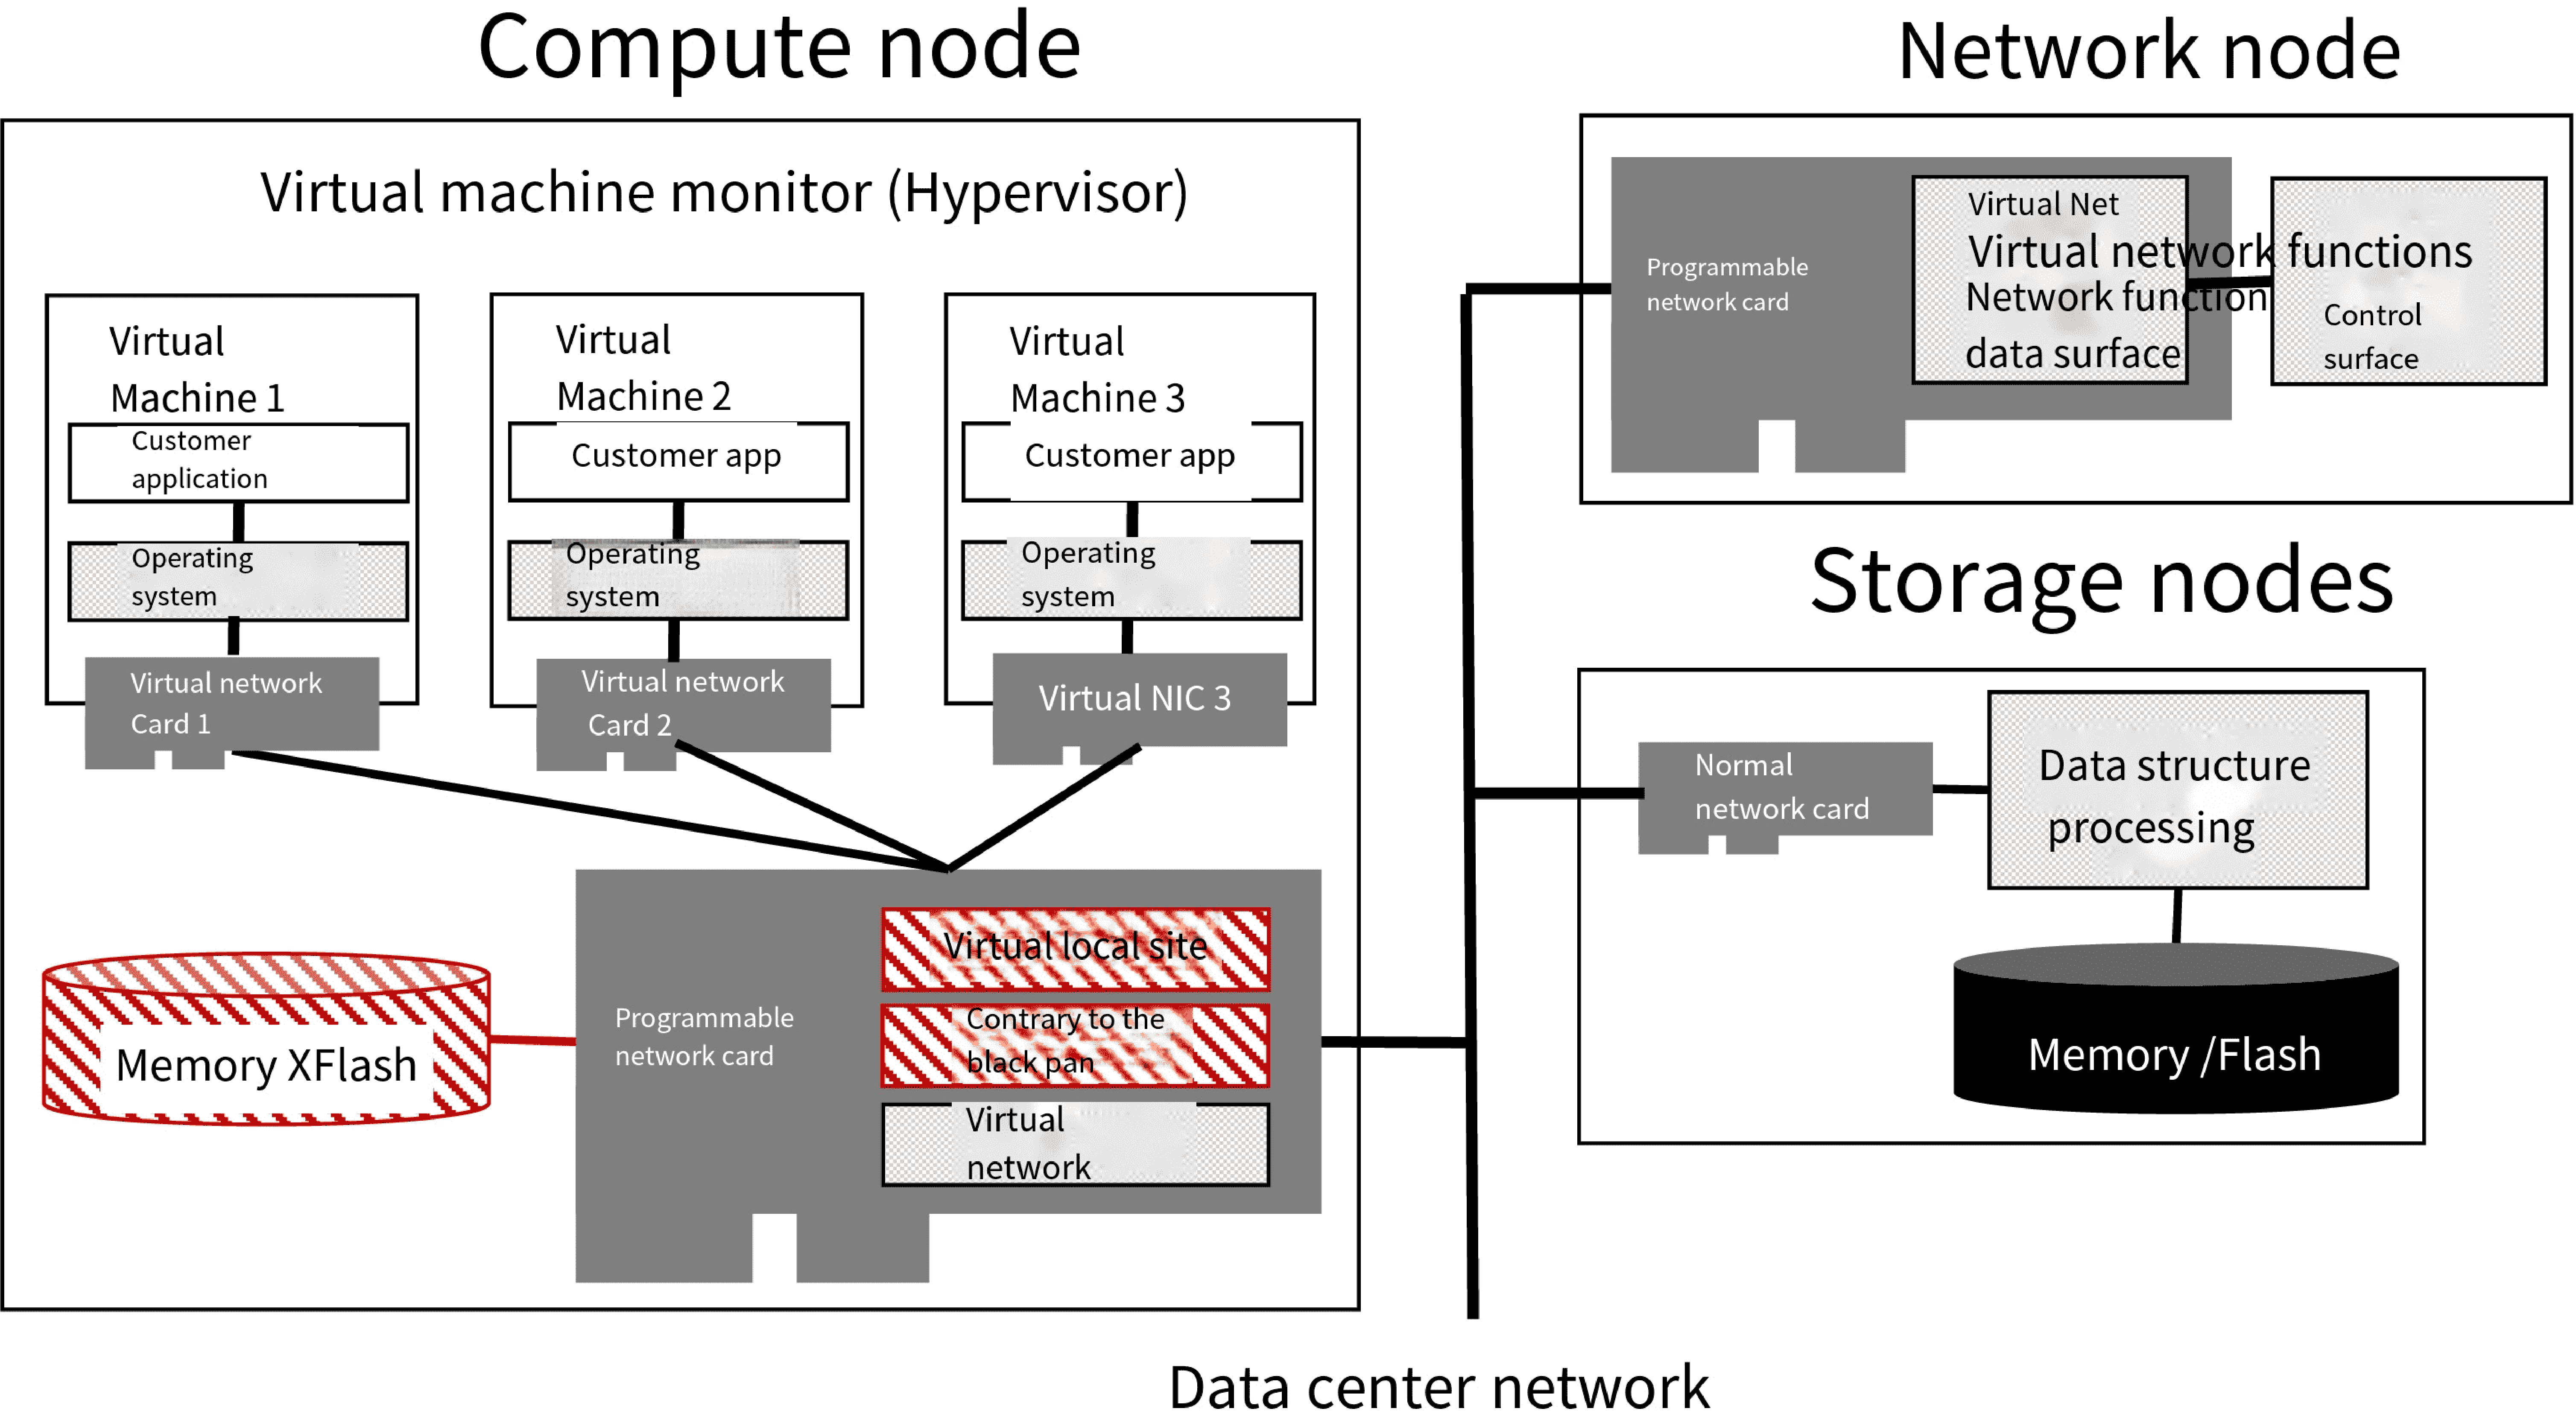
\includegraphics[width=0.8\textwidth]{figures/virt_storage.pdf}
	\caption{用可编程网卡加速本地存储和云存储后的架构。}
	\label{arch:fig:virt-storage}
\end{figure}

\subsection{数据结构处理加速}

数据面是操作相对频繁、逻辑相对简单的处理,而控制面是操作相对不频繁、逻辑相对复杂的处理。我们在可编程网卡中实现数据面,在主机 CPU 上实现控制面,实现了数据面完全不经过主机 CPU。

第 \ref{chapter:clicknp} 章的 KV-Direct 实现了多个客户端并发访问共享键值存储,并能保证一致性

网卡直接访问内存数据结构

直接访问远程硬件资源,而无需经过远程机器的 CPU。

\begin{figure}[htbp]
	\centering
	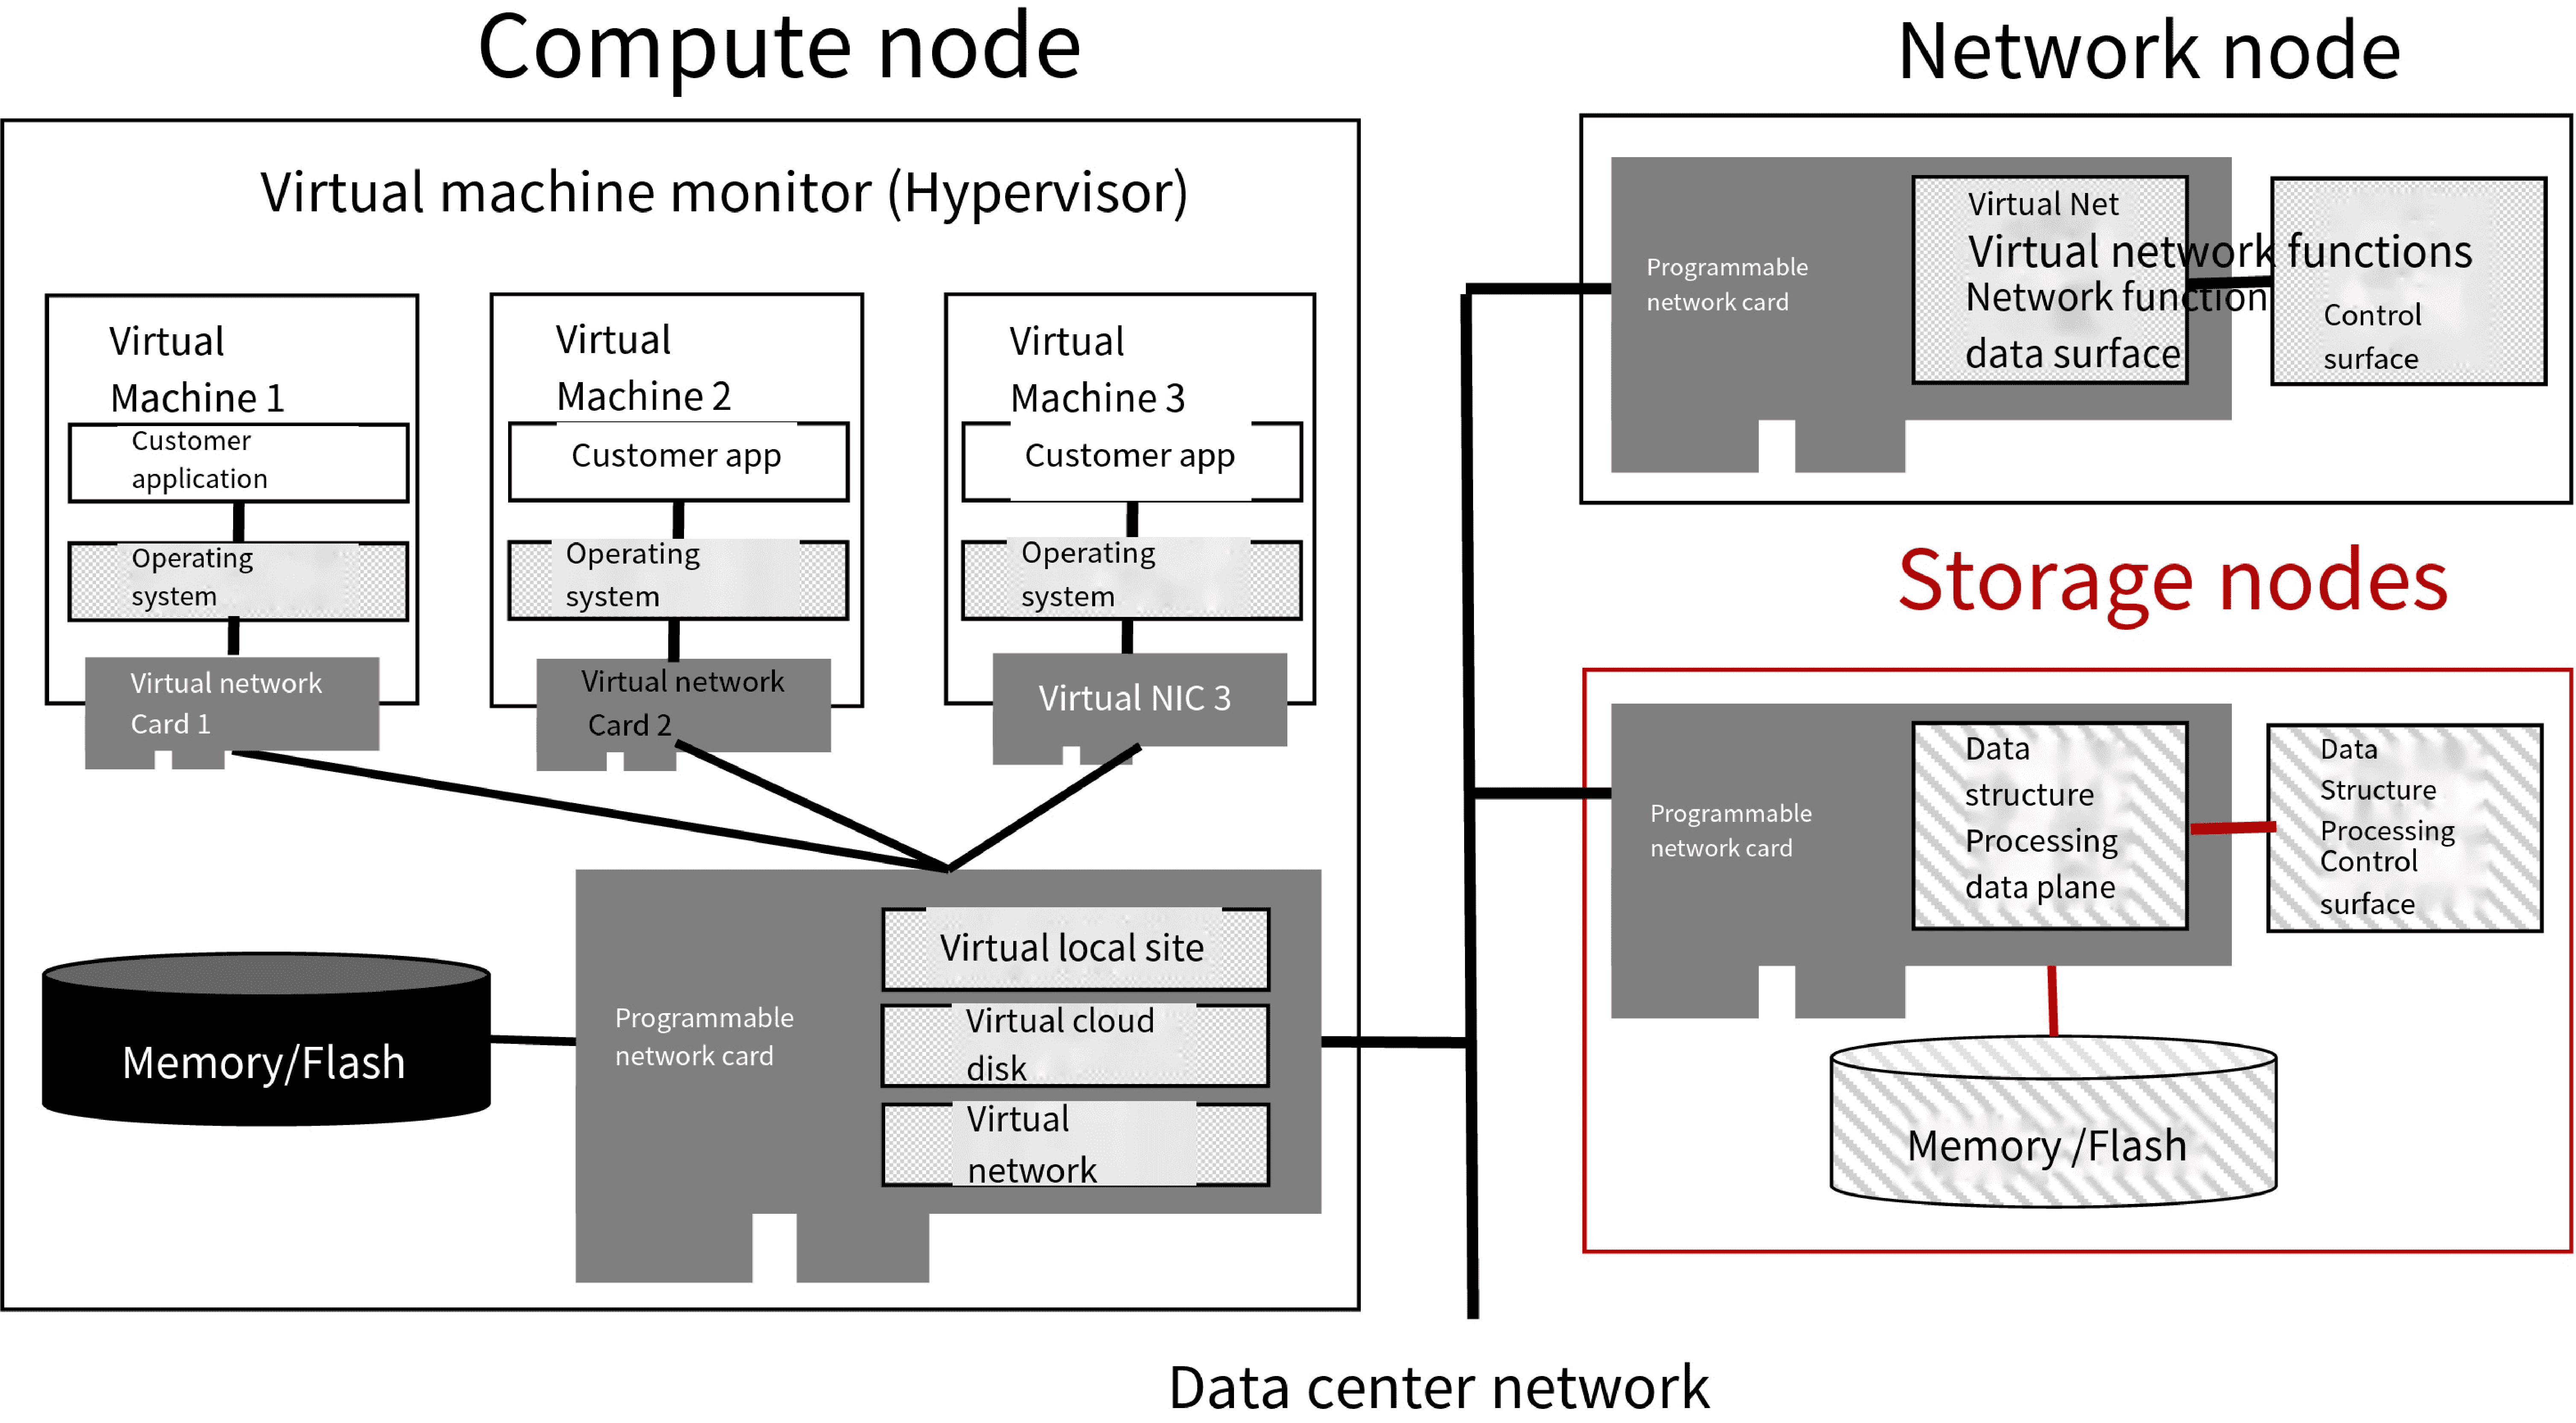
\includegraphics[width=0.8\textwidth]{figures/data_structure_accel.pdf}
	\caption{用可编程网卡加速数据结构处理后的架构。}
	\label{arch:fig:data-structure-accel}
\end{figure}

\section{操作系统加速}

可编程网卡上的可靠通信协议和主机 CPU 上运行的用户态库、用户态管理程序

OS kernel 给应用程序提供的原语可以重构为(控制面)协调和管理(仍在内核或用户态 daemon) + (数据面)用户态 library 负责高层抽象 + (数据面)可编程网卡负责多路复用、调度唤醒和可靠传输等低层语义,需要思考数据面上软硬件的接口(SocksDirect)。

客户应用程序如果可以使用云服务商提供的运行库和驱动程序,可编程网卡就不一定需要支持硬件虚拟化。例如第 \ref{chapter:socksdirect} 章的 SocksDirect 在用户态运行库中实现了套接字,其与网卡间的通信就不需要使用虚拟网卡,而只需与物理网卡建立通信队列。

\begin{figure}[htbp]
	\centering
	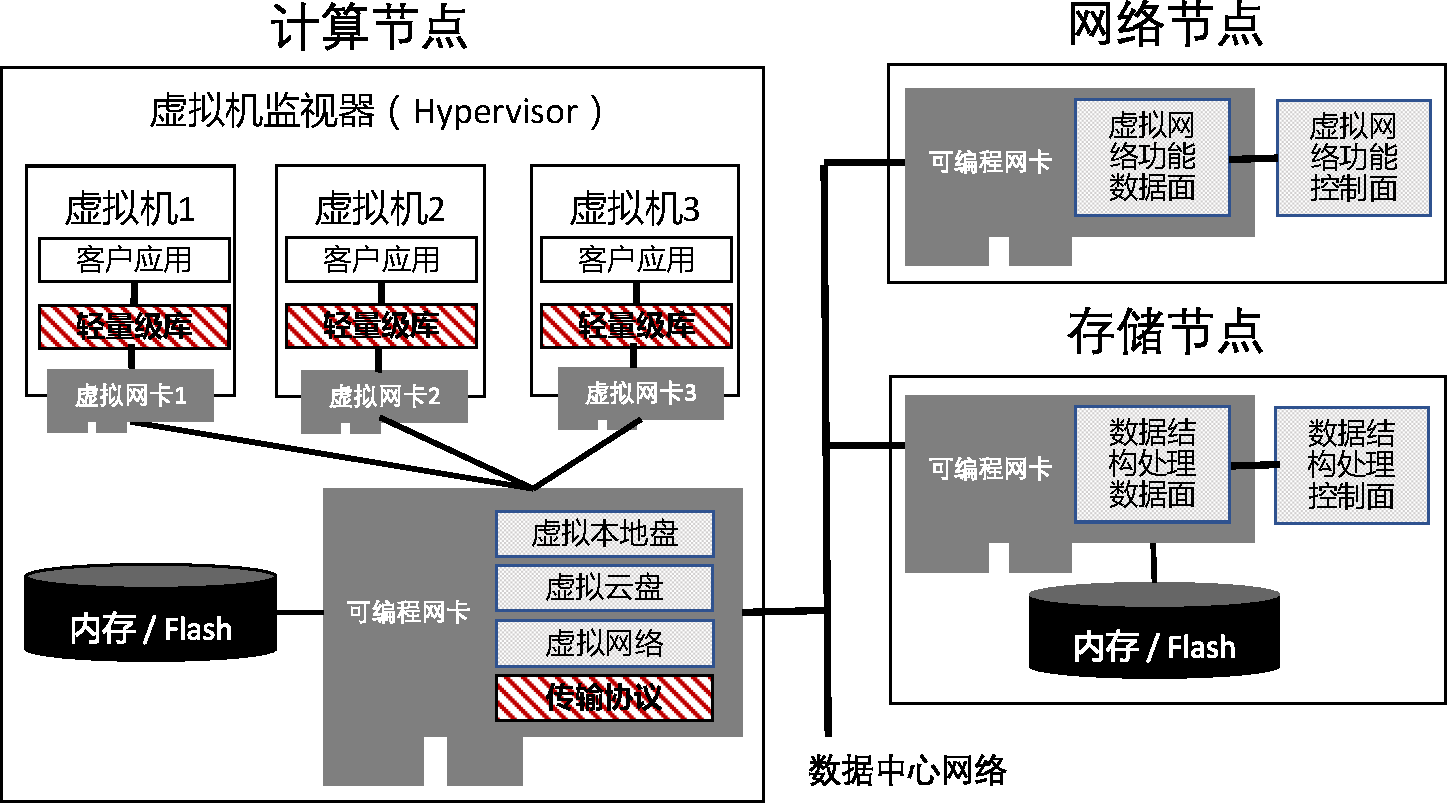
\includegraphics[width=0.8\textwidth]{figures/os_primitives_accel.pdf}
	\caption{用可编程网卡加速操作系统通信原语后的架构。}
	\label{arch:fig:os-primitives-accel}
\end{figure}


\section{可编程网卡}



\begin{figure}[htbp]
	\centering
	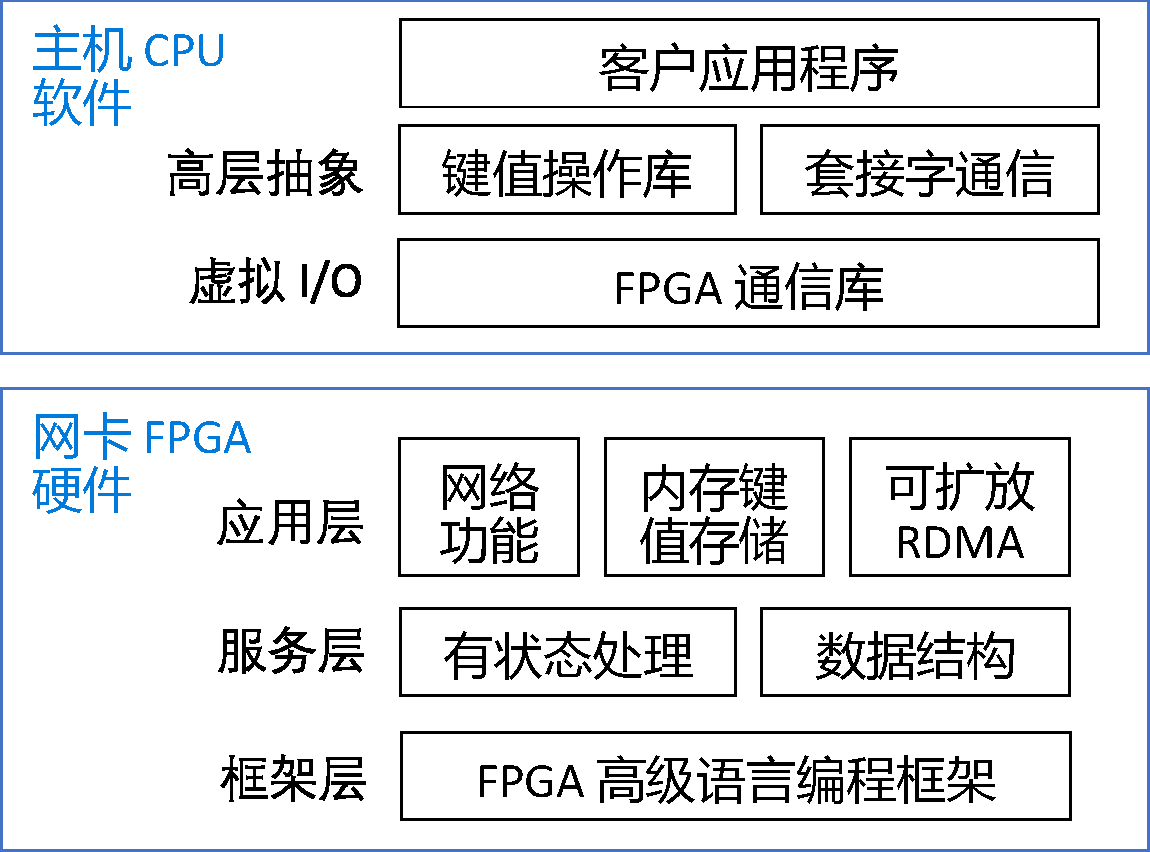
\includegraphics[width=0.6\textwidth]{figures/sw_hw_codesign.pdf}
	\caption{软硬件协同设计的可编程网卡架构。}
	\label{arch:fig:sw-hw-codesign}
\end{figure}


\subsection{硬件架构}

可编程网卡需要高度灵活性。为什么要 FPGA + CPU + ASIC SoC。回应第二章。

\textbf{图1: 网卡 SoC 结构图}

\subsection{高级语言编程框架}

FPGA 高级语言编程:ClickNP,适合流式处理的模块化 FPGA 高级语言编程

虚拟机热迁移,计算节点对应的网卡状态;网络、存储节点热迁移(升级,扩容等),网卡状态;高可用性,故障恢复……

\subsection{基础服务中间件}



第 \ref{chapter:kvdirect} 章提出的 FPGA 内有状态处理(stateful processing)、数据结构。
第 \ref{chapter:clicknp} 章的有状态网络功能、第 \ref{chapter:kvdirect} 章的内存键值存储、第 \ref{chapter:socksdirect} 章的可扩放 RDMA 的基础。
尽管第 \ref{chapter:clicknp} 章的 ClickNP 在第 \ref{chapter:kvdirect} 章之前发表,发表时的有状态处理和哈希表是使用与应用逻辑耦合紧密的方式实现的,既不容易扩放到大量并发连接,代码的可维护性也不强。
使用第 \ref{chapter:kvdirect} 章的 KV-Direct 作为基础后,这些网络功能的实现将变得模块化和可扩放。

本文使用高级语言编程框架实现基础服务中间件,中间件未来可以硬件化。
